

\section{Approach}\label{sec:approach}

The target of our method is to recover the missing contents in a corrupted video with fine details and temporal consistency.
%
We complete each frame by aggregating information for its neighboring frames. 
%Our intuition is that there exists complementary information in neighboring frames, which can benefit the inpainting process of each individual frame. Therefore,
In order to synthesize the missing content and produce a completed frame $\widetilde{V}_t$ at time $t$, we take total $T$ input frames $\boldsymbol{V}$ ($T=5$), indexed by $\msset{V}$, as input to our inpainting network in each data batch. 
%
The corrupted regions are indicated by binary masks $\boldsymbol{M}$ where $M_t^p=1$ indicates corrupted pixel $p$ in frame $V_t$. 
%

% 
%The corresponding ground truth frames are denoted as $\boldsymbol{V}^{gt}$.
%Our method infers each target frame $Y_t$ individually but with hints from its neighboring source frames.
%To fill up the missing region with structural details and temporal coherence,

The detailed network architecture is shown in 
Fig.~\ref{fig:stiNet}.
It consists of three main components. 
The first part is an edge inpainting network (ENet) for structure inference that recovers edge maps in the missing regions of the input frames.
The second part is a coarse-to-fine texture inpainting network (TexNet) that aims to complete the missing content with visual details under the guidance of hallucinated edges.
%which is much easier to hallucinate without complex colors.Therefore, under the guidance of well-completed object structure, we can better inpaint the whole texture.
The third part leverages the ground truth motion flow as auxiliary constraints to enforce temporal coherence of both the completed edge maps and textures at the training stage.
%The ground truth motion flow is employed to guarantee the consistency of edges and aggregate previously synthesized frames to refine the current frame.
%During the inference stage, only the edge-guided inpainting path is used to complete the target frame, which generates high-quality inpainted results with low time cost.


\subsection{Edge Inpainting Network}
\label{sec:edgenet}
%Before completing the missing texture in a piece of video, we first predict the sparse edges using an edge inpainting network (ENet).

The edge inpainting network (ENet) completes image edges in the missing regions to depict scene structures and object shapes.
Given the input corrupted frames $\boldsymbol{V}$ as well as the corresponding binary masks $\boldsymbol{M}$, a Canny edge detector is first applied to extract the corresponding edge maps $\boldsymbol{E}^{i}$ in the uncorrupted regions. %Notably, the edges in the masked regions in $\boldsymbol{E}^{i}$ are missed. 
%Given the incompleted grayscale images $\boldsymbol{X}^{g}$ of input frame, a canny edge detector is first used to generate initial edge maps. 
The input of ENet consists of the incomplete grayscale version of frames $\boldsymbol{V}^{g}$, initial edge maps $\boldsymbol{E}^{i}$, and their corresponding masks $\boldsymbol{M}$.
%
As shown in Fig.~\ref{fig:stiNet}, our ENet, denoted by $G^E$, is composed of a two-layer 3D encoder, eight 2D residual blocks, and a two-layer 3D decoder. 
The 3D encoder and decoder are designed to learn the spatio-temporal correlation with 3D convolution operations.
The intermediate 2D residual blocks are used to enlarge the spatial receptive fields by using 2D convolutions with large kernel size.
Such a hybrid 3D and 2D convolution architecture can achieve a good trade-off between spatial and temporal coherence.
The inpainted $T$ edge maps 	$\boldsymbol{\widetilde{E}}=\msset{\widetilde{E}}$ are obtained by:
\begin{equation}
	\label{eq:edgenet}
	\boldsymbol{\widetilde{E}}=G^E(\boldsymbol{E}^{i},\boldsymbol{V}^{g},\boldsymbol{M}).
\end{equation}

To train the edge generator $G^E$, ENet plays a minimax game by:
\begin{equation}
	\label{eq:loss_e_}
	\min\limits_{G^E} \max \limits_{D^E} \big(\mathcal{L}^E_{adv}+\lambda_1 \mathcal{L}^E_{fm}\big),
\end{equation}
where the discriminator $D^E$ follows the $70\times 70$ PatchGAN architecture \cite{Isola_2017_CVPR}. 
$\mathcal{L}^E_{adv}$ and $\mathcal{L}^E_{fm}$ are the adversarial loss and feature matching loss respectively. 
$\lambda_1$ is a hyper-parameter to balance the two terms.
%
In Eq.~\eqref{eq:loss_e_}, $\mathcal{L}^E_{adv}$ is an adversarial learning loss to make the predicted edge maps more realistic, which evaluates the image-level similarity between ground truth edge maps and the predicted edge maps by:
\begin{equation} \label{eq:edge_adver}
	\begin{aligned} 
		\mathcal{L}^E_{adv}  =&\mathbb{E}_{({E}^{gt},{V}^{g})}\big[logD^E({E}^{gt},{V}^{g})\big]\\ 
		+&\mathbb{E}_{({\widetilde{E}},{V}^{g})}\big[log\big(1-D^E ( {\widetilde{E}},{V}^{g})\big)\big].
	\end{aligned}
\end{equation}
% 
$\mathcal{L}^E_{fm}$ evaluates the feature-level similarity between ground truth and predicted edge maps, which is defined by:
%Feature matching loss was first proposed in \cite{wang2018high} and has been widely used in recent GANs.
%The feature matching loss is defined as:
\begin{equation}
	\label{eq:edge_fm}
	\mathcal{L}^E_{fm}=\sum_{t=1}^T\sum_{k=1}^L{\frac{1}{N_k}\left\| D^E_k({E}_t^{gt},{V}_t^{g})- D^E_k({\widetilde{E}_t},{V}_t^{g})\right\|_1},
\end{equation}
where $D^E_k$ is the $k$-th layer in the $L$-layer $D^E$, while $N_k$ is the element number of the output of $D^E_k$.
By considering both feature-level and image-level similarities in Eq.~\eqref{eq:loss_e_}, the edge generator $G^E$ can be trained to produce plausible and structurally rational edge maps.
%Note that the discriminator $D^E$ is not optimized by the feature matching loss term. It plays as a feature extractor to optimize the generator $G^E$ for producing plausible edge maps $\boldsymbol{E}$.

As a result, the proposed hybrid 3D and 2D convolution architecture and the two-level loss function enable the ENet to hallucinate the missing edges accurately.
An example of the generated edge map is given in Fig.~\ref{fig:coarse-fine} (a) and (b). 
The stripe pattern on the dog body is well inferred from neighboring frames. 


\begin{figure}[t]
	\centering
	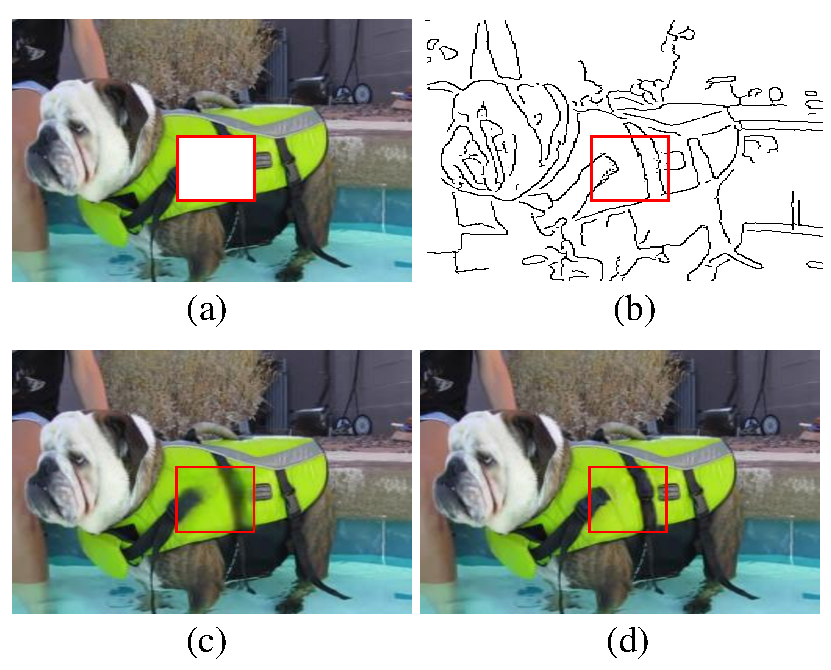
\includegraphics[width=0.8\columnwidth]{coars-fine} % Reduce the figure size so that it is slightly narrower than thre column. Don't use precise values for figure width.This setup will avoid overfull boxes. 
	\caption{To inpaint missing regions in a corrupted frame (a), our ENet first completes corresponding sparse edges (b), which well represent the structure of the missing contents. Then TexNet progressively replenishes textures under the guidance of synthesized edges from coarse (c) to fine (d).}
	
	\label{fig:coarse-fine}
\end{figure}




\begin{figure}[t]
	\centering
	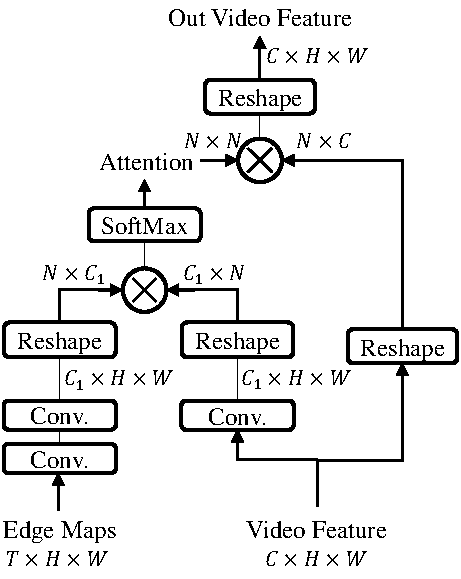
\includegraphics[width=0.65\columnwidth]{SEM} % Reduce the figure size so that it is slightly narrower than the column. Don't use precise values for figure width.This setup will avoid overfull boxes. 
	\caption{Architecture of the structure attention module. $C$ is the channel of the input video features, and $N=H\times W$. $\otimes$ represents matrix multiplication. Usually, we set $C_1=C/8$.}
	\label{SEM}
\end{figure} 




\subsection{Edge-Guided Texture Inpainting Network}

%Combining the inpainted edge maps $\boldsymbol{E}$ and flow maps $\boldsymbol{O}$, a spatio-temporal inpainting network (STINet) is designed to obtain the final target frame $Y_t$.

With the completed edge maps $\boldsymbol{\widetilde{E}}$ for the $T$ frames $\boldsymbol{V}$, we then fill the image texture using a coarse-to-fine network` TexNet.
%
Notably, the image structure,~\emph{e.g.,} object shapes, is well represented by the completed edge maps $\boldsymbol{\widetilde{E}}$.
Thus, it becomes easier to fill the missing texture with the structural guidance of $\boldsymbol{\widetilde{E}}$.

To synthesize realistic frame textures, our TexNet adopts a coarse-to-fine architecture, as shown in Fig.~\ref{fig:stiNet}.
Specifically, TexNet consists of a coarse inpainting network and a refinement network.
%
%The input of TexNet is the concatenation of  $\boldsymbol{\widetilde{E}}$, $\boldsymbol{V}$, and $\boldsymbol{M}$.
First, the coarse inpainting network consists of a set of 3D convolutions to capture the spatio-temporal information from the hallucinated edge maps and the corrupted input frames, and produces a rough completion $\boldsymbol{\widetilde{V}}^i$ for the $T$ frames with colors and textures.
%The 3D coarse network incorporates neighboring frames by convolutions of the time dimension.
Then, the refinement network takes the rough inpainting results $\boldsymbol{\widetilde{V}}^i$ and the synthesized edge maps $\boldsymbol{\widetilde{E}}$ as inputs to further refine texture details in $\boldsymbol{\widetilde{V}}^i$ with the guidance of structural edges $\boldsymbol{\widetilde{E}}$.
Notably, only 2D convolutional layers are used in the refinement network to improve the inference efficiency. 
%For the corrupted region, our ENet first completes sparse edges which well represent the structure of the missing content, then TexNet progressively replenishes textures under the guidance of synthesized edges.

Besides taking $\boldsymbol{\widetilde{E}}$ as an auxiliary input in the refinement network, we further design a structure attention module (SAM) to fully encode the structural information.
The detailed implementation of SAM is given in Fig.~\ref{SEM}.
% which is used as an intermediate layer in the refinement network in Fig.~\ref{fig:stiNet}.
The inputs of SAM are the intermediate video features extracted from $\boldsymbol{\widetilde{V}}^i$ and $\boldsymbol{\widetilde{E}}$ via 2D convolutional layers, as well as
the edge maps. %The output is a matrix that indicates the relationship among different spatial features.
%Two separate convolution blocks are first applied to embed structure features from the predicted edge maps $\boldsymbol{E}$.
% which alleviate the feature discrepancy between structural edge and video texture.
First, the intermediate video features and embedded edge features are interacted to calculate the latent structure-texture correlation via matrix multiplication. 
After a SoftMax operation, the normalized attention map is obtained while conveys the correlation between sparse structures and video features.
%
Then, the normalized attention map is applied to the intermediate video features, and the structure information is thus embedded in TexNet, which can better extract useful structural information brought by edges.
After introducing structural guidance in the refinement network, the inpainted content by TexNet becomes more realistic, as Fig.~\ref{fig:coarse-fine} (d) shows.

%The core insight of SAM is to explicitly capture the spatial correlation between edges and textures, which is regarded as a guidance in the texture generation processing.

%Fig.~\ref{fig:coarse-fine} shows an example of our structure-guided inpainting result. 

The coarse inpainting network and the refinement network in TexNet are trained as a whole, define by $G^T$, end-to-end in adversarial manner by:
%
\begin{equation}
	\label{eq:1}
	\min\limits_{G^T} \max \limits_{D^T} \big(\mathcal{L}^{T}_{rec}+\mathcal{L}^T_{adv}\big),
\end{equation}
where $D^T$ is the discriminator.
%, which has a similar architecture as $D^E$.
%
Inspired by \cite{nazeri2019edgeconnect}, the first term $\mathcal{L}^{T}_{rec}$ is the $l_1$-reconstruction loss to measure the difference between predicted video frames and the ground truth video frames $\boldsymbol{V}^{gt}$.
Differently, we penalize both the coarse predictions $\boldsymbol{\widetilde{V}}^i$ and refined frame $\widetilde{V}_t$, given by:
\begin{equation}
		\label{eq:loss_rec}
	\begin{aligned}
		\mathcal{L}^{T}_{rec}&=\frac{1}{\left\|M_t \right\|_1}\left\|(\widetilde{V}_t-V^{gt}_t)\odot M_t\right\|_1,\\ 
		&+\lambda_2*\frac{1}{\left\|\boldsymbol{M} \right\|_1}\left\|(\boldsymbol{\widetilde{V}}^i-\boldsymbol{V}^{gt})\odot \boldsymbol{M}\right\|_1,
	\end{aligned}
\end{equation}
where $V^{gt}_t$ denotes the ground truth frame at time $t$, and $M_t$ is the corresponding binary mask. 
%
%
Besides, an extra adversarial loss $\mathcal{L}^T_{adv}$ is introduced in Eq.~\eqref{eq:1} to promote the visual realism of the generated frame
 by:
	%$\mathcal{L}^I_{adv}$ is defined as:
	\begin{equation}
		\label{eq:inp_adver}
		\mathcal{L}^T_{adv}=\mathbb{E}[logD^T(V^{gt}_t)]+\mathbb{E}[log\big(1-D^T(\widetilde{V}_t)\big)].
	\end{equation}
$\mathcal{L}^T_{adv}$ enforces the generated frame to be more realistic.


The coarse and refinement networks can be effectively trained jointly with the combined loss of $\mathcal{L}^T_{rec}$ and $\mathcal{L}^T_{adv}$.
The results in Fig.~\ref{fig:coarse-fine} (c) and (d) show that the coarse network completes the missing content with rough structures and the refinement network exactly refines the inpainting results with more sharp contours and realistic textures.

% enables the TexNet to first give a coarse inpainting results, and then refine the results with the structure guidance.
%It can be seen that the coarse-to-fine architecture


 

\subsection{Flow-Guided Temporal Coherence Enhancement}
\label{sec:fec}
Besides the structural guidance, motion information is also considered to enhance temporal consistency among the recovered frames.
%It is vital to maintain temporal consistency in video inpainting.
%Optical flows are widely used to represent the dense correspondence between frames.
%To enhance temporal consistency in the synthesized results
To this end, we employ optical flow in the training stage of both ENet and TexNet.
%smooth the inpainted edge maps and synthesized frames in ENet and TexNet.
% and reinforce the temporal coherence between neighboring edge maps and frames during training. 
%Moreover, we design an ensemble module that leverages the previous inpainted frames to refine the current frame completion, as Fig.~\ref{fig:stiNet} shows. 
%
A set of flow maps \(\boldsymbol{O}\) between the current frame $V_t^{gt}$ and its neighboring frames are generated using a pre-trained flow extraction network, such as FlowNet2.0~\cite{Flownet_2017_CVPR}.
Specifically, \(\boldsymbol{O}\) consists of four flow maps \((O_{t\Rightarrow t-7}, O_{t\Rightarrow t-3}, O_{t\Rightarrow t+3}, O_{t\Rightarrow t+7})\).
%\(\boldsymbol{O}\) contains the ground truth motion information between frames, which is important to both edge and texture generation.

%From the predicted optical flow $\boldsymbol{O}^i$, FNet estimates the flow in the missing regions to obtain four flow maps \(\boldsymbol{O}\) as:
%\begin{equation}
%	\label{eq:flownet}
%	\boldsymbol{O}=G^F(\boldsymbol{O}^{i},\boldsymbol{M}),
%\end{equation}
%where $G^F$ denotes FNet, which consists of an encoder that uses ResNet101 \cite{He_2016_CVPR} as backbone and a decoder.
%The detailed architecture of FNet is shown in Fig.~\ref{fig:stiNet}.


In terms of the ENet which completes the missing edges, \(\boldsymbol{O}\) is used to first warp the neighboring edge maps to the current frame, and then compute the consistency between neighboring edge maps. 
%
%Instead of separately training two subnetworks ENet and FNet, we train them jointly, because the temporal correlation and structural details can boost each other. 
Thus, a flow-guided edge consistency loss is defined as:
%
\begin{equation}
	\label{eq:flow_edge}
	\mathcal{L}^E_{fec}=\sum_{k}\frac{1}{\left\|M_{t} \right\|_1}\left\|\big(\widetilde{E}_{t}-\phi(O_{t\Rightarrow t+k},E_{t+k}^{gt})\big)\odot M_{t}\right\|_1,
\end{equation}
where $\phi(O_{t\Rightarrow t+k},E_{t+k}^{gt})$ is the warping operation which warps the edge map $E_{t+k}^{gt}$ to the target frame according to the generated optical flow $O_{t\Rightarrow t+k}$.
$k$ denotes the index of neighboring frames ($k\in \left\{-7,-3,+3,+7 \right\}$). 
With the flow-guided edge consistency loss $\mathcal{L}^E_{fec}$, the loss function of  Eq.~\eqref{eq:loss_e_} for ENet becomes:
\begin{equation}
\label{eq:loss_e}
\min\limits_{G^E} \max \limits_{D^E} \big(\mathcal{L}^E_{adv}+\lambda_1 * \mathcal{L}^E_{fm}+\mathcal{L}^E_{fec}\big).
\end{equation}

\dlt{The total loss function for the FNet is given by:
\begin{equation}
	\label{eq:flow_all}
	\mathcal{L}_{flow}=   \mathcal{L}^F_{rec}+ \mathcal{L}^F_{har}+\mathcal{L}_{fec},
\end{equation}
where $\mathcal{L}^F_{rec}$ and $\mathcal{L}^F_{har}$ are respectively $l_1$ loss and hard example mining loss in the missing regions, following the definition in \cite{Xu_2019_CVPR}.} 
%Specifically, $\mathcal{L}^F_{har}$ encourages the network to focus on those hard samples in order to avoid blurry texture.

%Specifically, $\mathcal{L}_{fec}$ warps the edge maps from neighboring frames to the target frame to penalize the reconstruction loss.
%In terms of ENet, $\mathcal{L}_{fec}$ encourages the predicted edge maps to be temporally smoothing, which should conform to the motion tendency in the flow maps $\boldsymbol{O}$. 
%In terms of FNet, $\mathcal{L}_{fec}$ constrains the model to focus on edges.
%Thus, the total loss function for joint training of ENet and FNet is:
%\begin{equation}
%    \label{eq:flow}
%    \mathcal{L}_{joint}=\mathcal{L}_{edge}+\mathcal{L}_{flow}+ \mathcal{L}_{fec}.
%\end{equation}


About the TexNet, we further enforce the temporal coherence of synthesized neighboring textures via a flow warping constraint $\mathcal{L}^T_{flo}$ by: 
\begin{equation}
	\label{eq:inp_flow}
		\mathcal{L}^T_{flo}=\sum_{k}\frac{1}{\left\|M_{t} \right\|_1}\left\|\big(\widetilde{V}_{t}-\phi(O_{t\Rightarrow t+k},V_{t+k}^{gt})\big)\odot M_{t}\right\|_1,
	\end{equation}
where  $k$ is also in $\{-7,-3, 3, 7\}$. $\phi(O_{t\Rightarrow t+k},V_{t+k}^{gt})$ warps $V_{t+k}^{gt}$ to the target frame using flow $O_{t\Rightarrow t+k}$. Finally, $\mathcal{L}^T_{flo}$ is added to Eq.~\eqref{eq:1}, which becomes:
\begin{equation}
\label{eq:1_}
\min\limits_{G^T} \max \limits_{D^T} \big(\mathcal{L}^{T}_{rec}+\mathcal{L}^T_{adv} +\mathcal{L}^T_{flo}\big).
\end{equation}

After adding the motion information to both the training process of ENet and TexNet, the temporal consistency can be enhanced in both edge generation and texture inpainting.
Since the motion is only used in the training stage, the inference of the proposed structure-guided inpainting method is efficient and effective.

%Finally, a temporal ensemble module is designed to refine the current frame $Y_t$ by aggregating previous frames. %The architecture is shown in Fig.~\ref{fig:stiNet}. 
%This module is trained with a $l_1$-reconstruction loss and an adversarial loss.







	